\openingarticle
\def\ppages{\pagerange{thoeming:firstpage}{thoeming:lastpage}}
\def\shorttitle{Dealing with Data}
\def\maintitle{Dealing with Data: Naïve Bayesian Classification  and a Case Study from  Viking Age Sweden}
\def\shortauthor{Alix Thoeming }
\def\authormail{alix.thoeming@sydney.edu.au}
\def\affiliation{Department of Archaeology, The University of Sydney}
\def\thanknote{\footnote{Alix Thoeming is a PhD candidate in the department of Archaeology at the University of Sydney, having previously completed her undergraduate degree at the same university, graduating with first-class honours. Alix’s PhD thesis will explore urban trajectories within Eastern and Northern Europe after the decline of the Roman Empire, though she has developed a strong interest in exploring alternative methodologies for use with archaeological data, specifically those derived from mathematics and computer science. She was the first recipient of the Bruce G. Trigger Award for Archaeological Thought at NASC 2014 for her presentation about her honours thesis, which inspired the present article.}}
%--------------------------------------------------------------
\mychapter{\maintitle}
\begin{center}
	{\Large\scshape\shortauthor\thanknote}\\[1em]
	\email \\
	\affiliation
\end{center}
\vspace{3em}
\midarticle
%--------------------------------------------------------------
	\label{thoeming:firstpage}
\begin{myabstract}
		Mathematical\marginnote{Abstract\\(in Swedish see below)} analysis is becoming ever more useful when dealing with large amounts of archaeological data, due to the precision and certainty with which results can be produced. This article will discuss the use of a relatively new tool in deciphering and dealing with archaeological data, the Naïve Bayes Classifier. The ‘Bayesian’ approach was first proposed in the early 1990s, by archaeological statistician Clive Orton \parencites[139]{Orton_1992}[1]{Buck_1996}, though at that time the lack of computational power available made use of the Classifier prohibitively difficult. Today a Naïve Bayes Classifier can be employed by anyone with a computer, without any need for particularly specialised computer skills. Programs such as Orange use a graphical interface as a way to circumvent the need for specific mathematical knowledge of the process, and the use of this program is detailed in the paper. The Naïve Bayes Classifier is most useful in attempting to identify unseen patterns in a large amount of data, such as a database with thousands of entries, and potential uses will be illustrated here. This paper presents a case study using a Naïve Bayes Classifier in an attempt to date Swedish Viking-age rune-stones, which remain undated through conventional methods. Two variables were identified as showing some small trace of temporal evolution, the Christian crosses and runic inscriptions on the stones, and the Classifier was utilized to explore their further use.
		
\keywords[Keywords]{Bayesian Statistics, Archaeological Statistics, Naïve Bayes Classifier, Archaeological Methodology, Quantitative Methods.}

	\end{myabstract}
	

	
%	\section{Introduction}
	
\lettrine[nindent=0em,lines=3]{A}{s} archaeologists we use mathematical tools in every stage of our profession, from calculating the minimal number of individuals in faunal assemblages, to assessing the likely use of whichever trench or square we are working with based on artefact appearance, to presenting and analysing results. Advanced mathematical methods, however, are often not explored until postgraduate study, and are in many situations and for many reasons avoided even then. A certain amount of advanced mathematical (generally statistical) literacy must be expected of archaeologists, and in particular of up-and-coming archaeologists. Moving from descriptive to inferential statistics is much less of a stretch than may be thought. This paper aims to demonstrate this by detailing the use of a tool that comes under the umbrella of Bayesian statistics, known as the Naïve Bayes Classifier. While descriptive statistics have traditionally been the most widely-used form of statistical analysis, ‘description…is not to be confounded with inference’ \parencite[5]{Buck_1996}, and from there comes a place for a tool such as the Classifier. 

	The Naïve Bayes Classifier is a tool using Bayes’ Theorem to summarise prior information from known information within a dataset into a qualitative model that may or may not have the strength to derive probabilistically significant conclusions to ‘fill out’ a dataset with unknown properties. It is best utilised when one class or feature within the given dataset is incomplete. The dataset should ideally have at least one thousand ‘objects’ - though this is just the author’s opinion, as it has proved possible with less - with at least 30\% of the objects having a value assigned to the target category. A case study attempting to date Swedish Viking-age rune-stones is laid out here to show just how easy the use of inferential statistical tools such as the Naïve Bayes Classifier has become. 

%	\section{Bayesian Theory in Archaeology}
	
	Bayesian\marginnote{Bayesian Theory in Archaeology} logic is a process familiar to all of us; every day we make choices, and many of those choices require us to reason towards the likely outcome of a given hypothesis. Developed in the early 18th century by Thomas Bayes, this theory was the first to establish a mathematical approach towards the inference of probability \parencite[2]{Delampady_2003}. The core principal of Bayesian analysis, that prior knowledge or information can be used to make an informed decision about that which is not yet known or understood, has been used archaeologically in many ways. While the earliest suggestion found of the use of Bayesian method within archaeology dates to the early 1970s \parencite[446]{Doran_1972}, they were not implemented in this discipline until the mid-1990s. This was primarily due to both certain unfriendliness in the available software, as well as its ‘ferociously heavy computational needs’ \parencite[139]{Orton_1992}. A book directed towards archaeologists was published at this time \parencite{Buck_1996}, outlining the basic concepts of Bayesian statistical methods and many situations to which they are suited. While the \textcite{Buck_1996} volume does discuss the use of Bayes’ theorem, the mathematical rule upon which a Naïve Bayes Classifier is based, the Classifier itself is not explicitly mentioned. Traditional Bayesian statistical studies have been much more wide-ranging; for example, the construction of Bayesian chronologies to calibrate radiocarbon dates \parencites{Bayliss_2007}{Levy_2010}(also see \textcite{Bayliss_2009}, for a detailed history of the process), Bayesian approaches and solutions to seriation problems \parencite{Halekoh_2004}, and even Bayesian assessments of the demagnetisation of limestone \parencite{Borradaile_2003}.
	
	Recent studies explicitly detailing the use of a Naïve Bayes Classifier in their methodologies include a 2006 publication examining the identification of regionally differentiated features in Levantine ivory sculptures \parencite{Gansell_2006}. Several features noted as having been overlooked were then identified in this study as regionally significant for classifying sculptures. A study exploring the prehistoric Mexican site of Monte Albán utilised a hybrid of the Classifier and a decision tree \parencite{Reynolds_2008}, and another presented its use in image differentiation, by breaking down heritage images into colour-differentiated pixel maps \parencite{Polpinij_2010}.
	
	While Bayesian statistics are generally used for large multivariate problems \parencite[129--134]{Buck_1996}, the Naïve Bayes Classifier is suitable for specific problems involving inferences concerning a single feature or class of artefact. This simplicity of design and implementation makes the Classifier an ideal starting point for archaeologists wishing to explore advanced statistical methods. It is also important to note that one of the main differences between Bayesian statistics and the Naïve Bayes Classifier is its use of conditional independence, an assumption that variables exist independently of each other, i.e. that the existence of attributes are not interrelated \parencite[231]{Tan_2006}\footnote{It should be noted that this text is an exceptional resource for anyone new to computational statistical methods, and is highly recommended as a reference text.}. 
	
%	\section{Using the Naïve Bayes Classifier}
	
	A Naïve\marginnote{Using the Naïve Bayes Classifier} Bayes Classifier is best utilised when there are ‘knowns’ –states of partial understanding \parencite[192]{Orton_1992} - that can be used to train the Classifier to calculate the probability of an individual object belonging to a pre-defined class. It is important to note that no Classifier can give a solid ‘yes’ or ‘no’ to any single object belonging to each of the classes or features within the target category; it can only offer a probability \parencite[235]{Tan_2006}. The mathematical theory at the root of the Classifier is Bayes’ Theorem (Fig. \ref{fig:Fig1}). Results from the Classifier (posterior beliefs) come about through combining the information already present (prior beliefs) and their statistical significance (standardised likelihoods) into a quantitative model. A Naïve Bayes Classifier is essentially a somewhat more sophisticated version of the coin-toss problem (calculate the probability of tossing 3 ‘heads’ in a row; 0.5\textsuperscript{3}=0.125). 
	
		%% this is FIGURE 1
		\begin{figure}[!htb]
			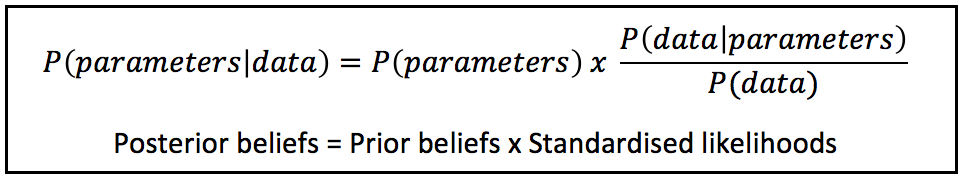
\includegraphics[width=\linewidth]{figures/thoeming_Fig1}
			\centering
			\caption{Bayes’ Theorem; adapted from \textcite[5]{Bayliss_2007}.}
			\label{fig:Fig1}
		\end{figure}	
	For example, the Bayesian model could be employed by a museum in deciding whether or not to purchase a southern Italian Apulian krater with a mythical scene at auction, given the unknown variable of reliable provenance (Fig. \ref{fig:Table1} or Table 1). This particular type of pot is not represented in the ‘known’ data set, which includes a field stating the reliability of provenance, and so we can use this data to calculate our odds. These data are used to provide the Classifier with the base information required to make an informed decision about our new Apulian krater. The evaluation provided by the Bayes rule gives us the conclusion that the likelihood of our new pot’s provenance being reliable is 0.037, and the likelihood of it not being 0.069. Given that 0.069>0.037, our example is classified into the ‘no’ category. The museum now has the choice as to whether or not accept these odds and risk purchasing the krater anyway. When used in an example such as this, the Classifier is run twice, first to assess the likelihood that our answer is ‘no’, and then to assess the likelihood that it is ‘yes’. In more complicated examples the Classifier would be run as many times as there are possible outcomes.
	
	%% this is FIGURE 2 Table 1
	\begin{figure}[!htb]
		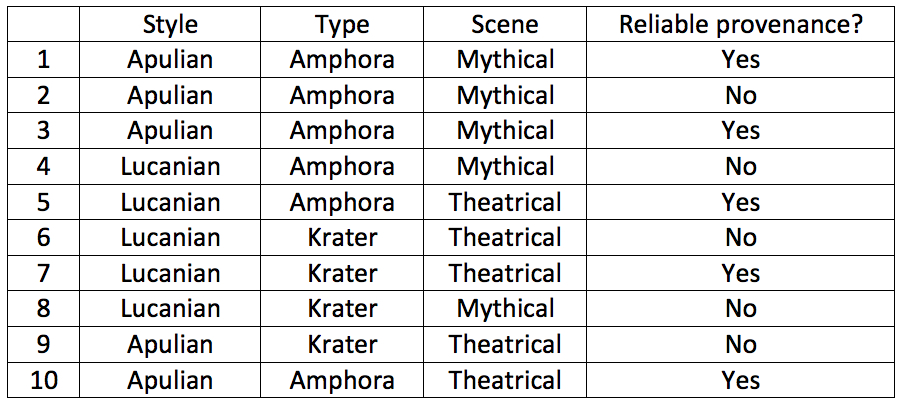
\includegraphics[width=\linewidth]{figures/thoeming_Table1}
		\captionof{table}{Naïve Bayes Classifier Example; adapted from \textcite{Meisner_2003}.}		
		\label{fig:Table1}
	\end{figure}
	When setting up data for use in a Classifier, it must be presented in a format similar to either Figure \ref{fig:Table1} (Table 1), or the more complex case study presented in section six. The data must be consistent; the Classifier would view a pot with the feature ‘Apulian’ as discrete from one labelled ‘APULIAN’ and different still from one labelled ‘apulian’. As each feature is treated entirely independently, the user must be especially careful about correctly informing the Classifier of all information provided in the dataset. Scale is irrelevant – this could be just as easily used for single artefacts as for large-scale settlements. It is possible to configure readable data in many different ways, but the key to reliable results is consistence in these data. The Classifier will not identify the value ‘75’ as any closer to ‘76’ than the value ‘234’, so if the user is, for example, measuring the size of objects, a range or ‘class’ (e.g. ‘small’, ‘medium’, or ‘large’), would be more useful.
	
%	\section{Assessing the Reliability of the Classifier}
	
	Traditionally\marginnote{Assessing the Reliability of the Classifier} statistical reliability has been tested through the t-test for statistical significance. The Naïve Bayes Classifier instead utilises two alternate tests to predict the reliability of its results. Both of these use cross-validation, in which the ‘known’ dataset (as opposed to the ‘unknown’ dataset, from where our results will come) is tested against itself in order to check the validity of its results. While a cross-validation can be run as few or as many times as the user desires, ten is the generally-accepted standard, and so it is therefore known as a ten-fold cross-validation. In this ten-fold cross-validation, the ‘known’ dataset is split into ten equal sections. Nine of these are chosen to ‘train’ the Classifier, with the remaining 10\% used as test data. The validation is then run until each segment has been used in a test capacity \parencite[187]{Tan_2006}. 
	
	The first of these tests is the confusion matrix, a standard tool for evaluating classification models. It provides the user with an approximation of the accuracy of the results of the Classifier, by simply dividing the number of correct predictions by the total number of predictions \parencite[149]{Tan_2006}(Fig. \ref{fig:Table2} or Table 2).
	
		%% this is FIGURE 3 Table 2
		\begin{figure}[!htb]
			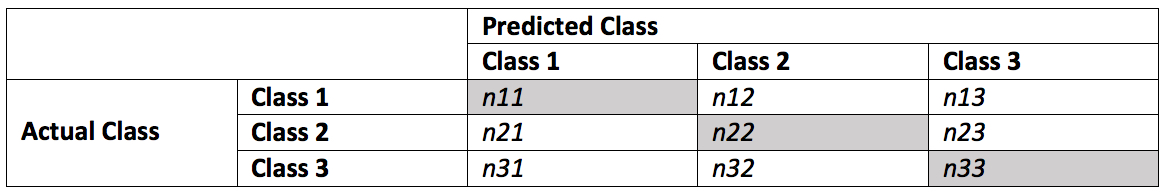
\includegraphics[width=\linewidth]{figures/thoeming_Table2}
			\centering
			\captionof{table}{Example Confusion Matrix.}		
			\label{fig:Table2}
		\end{figure}	
	The second test that provides an estimate of the Classifier’s accuracy is the ROC (receiver operating characteristic) curve. A ROC curve is a visual representation of the results that plots their true vs. false positive rates on a simple graph, forming a line of best fit through the results cluster. It summarises the information provided in the confusion matrix into four groups; true positive, false positive, true negative, and false negative. These groups are then calculated into a True Positive Rate (TPR) and a False Positive Rate (FPR). These represent the instances in which each individual object is classified correctly or incorrectly into each of the classes, with TPR represented on the Y–axis and FPR on the X–axis \parencite[298--301]{Tan_2006}(Fig. \ref{fig:Fig2}).
	
	%% this is FIGURE 4 (Fig 2)
	\begin{figure}[!htb]
		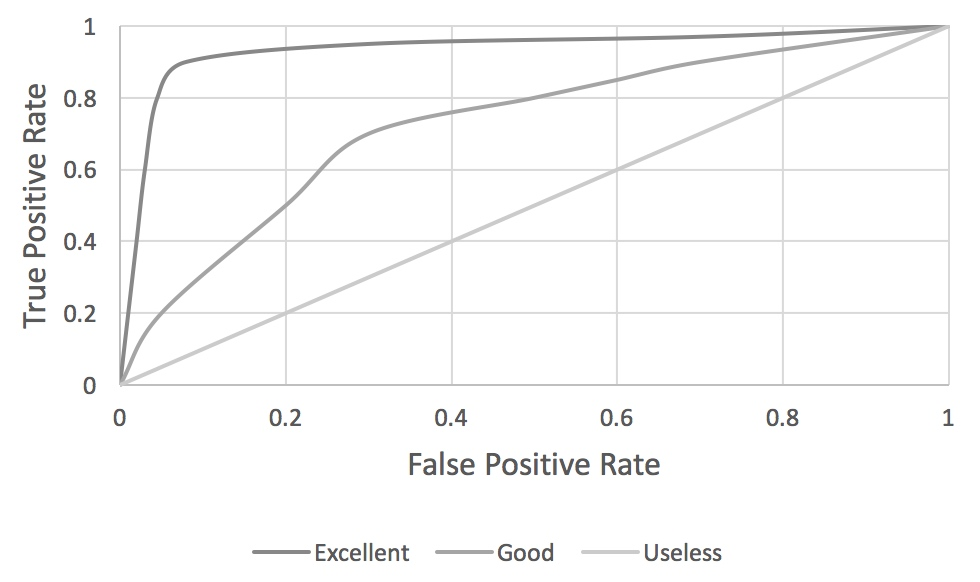
\includegraphics[width=.85\linewidth]{figures/thoeming_Fig2}
		\centering
		\caption{Example ROC (receiver operating characteristic) Curve.}
		\label{fig:Fig2}
	\end{figure}
	The results of a Naïve Bayes Classifier are typically produced in spreadsheet form, though they can be summarised by a graphical form\footnote{See \textcite[490]{Gansell_2006} for an example of nomographic representation.}. These results can only be considered reliable if the results of the two reliability predictors above satisfy the set minimum acceptable standard. The tabulated results assign a percentage to the probability of each individual object belonging to each of the specified classes, with the conclusion generally being that the class assigned the highest percentage is the correct prediction (Fig. \ref{fig:Table3} or Table 3).
	
	%% this is FIGURE 5 Table 3
	\begin{figure}[!htb]
		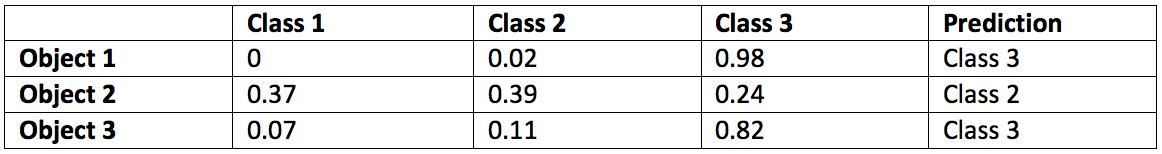
\includegraphics[width=.95\linewidth]{figures/thoeming_Table3}
		\centering
		\captionof{table}{Example Results Table.}		
		\label{fig:Table3}
	\end{figure}
	
%\section{Rune-Stones and Their Context}

Rune-stones\marginnote{Rune-Stones and Their Context} are large, shaped stones raised during the Viking Age to commemorate the life of a well-regarded individual. Typically somewhere between five and eight feet tall, they are the work of professional carvers who integrate a runic inscription (naming the deceased and their deeds, the sponsor(s), as well as in some cases themselves) that winds either within or around a stylised ‘rune animal’ of some sort, variously described as a dragon, serpent or bird, and in around half of all stones a Christian cross \parencite[10]{Sawyer_2000}. Sporadically erected before the end of the \nth{10} century \AD, the major period of activity in stone-raising was the \nth{11} century \AD This time period is traditionally seen as the tail end of the Viking Age, and while the raising of the rune-stones is surely causally related to the ‘viking’ activity taking place at the time (the word ‘viking’ itself is problematic; it has no modern equivalent, but is generally accepted to have been a verb, describing elite trading and occasional raiding. The term has since then undergone normalization, becoming a noun describing a horned-helmeted ‘barbarian’ \parencite[56]{Jesch_2001}, they are much more a product of the small elite ‘stay-at-home’ population than the Vikings themselves. These elites owned land and perhaps held some form of lordship over their locality \parencite[36--41]{Jesch_2001}, as well as potentially having a role in staking claims of inheritance \parencite[74--91]{Sawyer_2000}.

The rune-stones are very important in an archaeological discussion of the Christianisation process that was taking place at this time. In Sweden the process occurred relatively later than in Denmark and Norway and was much more fraught. It is seen as having occurred relatively quickly in the south of Sweden where the rune-stone fashion had faded by the middle of the \nth{10} century \parencite[501]{Lager_2010}, but faced much more opposition in the north, especially in the most populous region of Sweden at the time, Uppland (corresponding today to the greater Stockholm area). The response here to the ‘stubborn paganism’ of the region \parencite[39]{Herschend_1994} seems to have been a deliberate upswing –especially in the raising of ‘Christian’ rune-stones– around 1070 \parencite[501]{Lager_2010}. These ‘Christian’ rune-stones are identified in several ways, most commonly either through the integration of a Christian cross into the carved design of the stone, or through the use of a Christian phrase. Around 3,000 rune-stones have been documented in Scandinavia, with 250 in Denmark, 50 in Norway, and the rest in Sweden. This study only incorporated rune-stones from Sweden (Fig. \ref{fig:Fig3}), as their large number and well-documented presence in the runic inscriptions database Rundata allows for the measurement of a large number of variables.

%% this is FIGURE 6 (Fig 3)
\begin{figure}[!htb]
	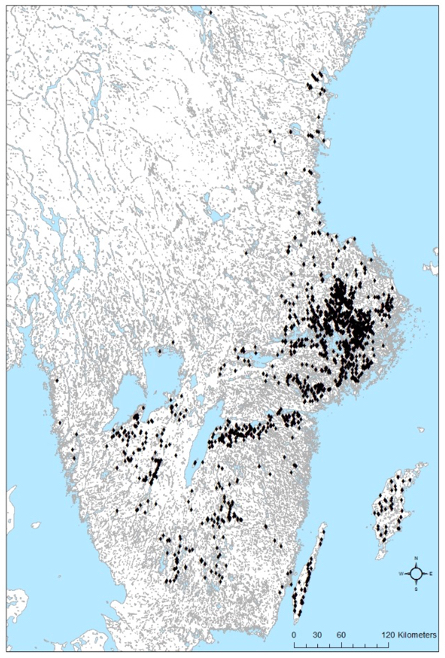
\includegraphics[width=.95\linewidth]{figures/thoeming_Fig3}
	\centering
	\caption{The Viking Age rune-stones of Sweden included in the study.}
	\label{fig:Fig3}
\end{figure}

%\section{Parameters of the Case Study}

The\marginnote{Parameters of the Case Study} primary aim of this study was to investigate whether it was possible to apply the Naïve Bayes Classifier to date the $\sim$40\% of rune-stones that remain undated through traditional methods. As stone artefacts, it is impossible to apply ‘absolute’ methods of dating, and while paint traces remain on several rune-stones, there are generally not sufficient enough organic binding agents remaining for the employment of C-14 dating \parencite[22]{Kitzler_2002}. The currently accepted dating scheme combines historical dates referenced in the runic inscriptions, the dates known for the carvers who signed their rune-stones, and a stylistic sequence which identifies changes in the carved ornamentation on the stones \parencite{Gräslund_2006}(Fig. \ref{fig:Table4} or Table 4).

	%% this is FIGURE 7 Table 4
	\begin{figure}[!htb]
		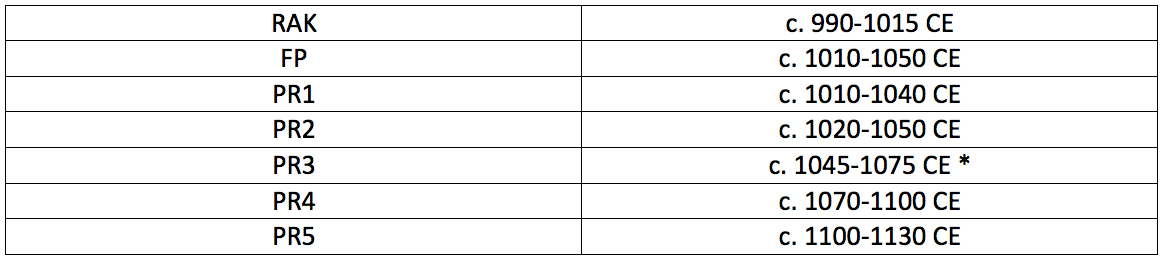
\includegraphics[width=.95\linewidth]{figures/thoeming_Table4}
		\centering
		\captionof{table}{Gräslund’s rune-stone dating; after \textcite{Gräslund_2006}. *Gräslund notes the end date for ‘PR3’ as being en generation framåt (a generation forward), which is here and in other literature \parencite[196]{Sawyer_2000} accepted to be around 30 years.}		
		\label{fig:Table4}
	\end{figure}

As previously mentioned, two variables were selected for analysis, but due to the results being quite similar this paper only discusses the results from analysis of the crosses on the stones. These crosses are seen in just under half of the Swedish rune-stones. \textcite{Lager_2002} proposed a classificatory system for these symbols, assigning each rune-stone a designation based on 51 sub-classes of seven main groups, each identified by both a letter and number. Lager detected a small amount of temporal differentiation in some of these features, noting that some appear only on earlier rune-stones, and that simpler crosses seem to appear in the later of Gräslund’s phases. Each cross is generally assigned several of the features based on its appearance; for example, a cross may as an example be given the designation ‘A1;B3;C8;C9;D1;F3’. 

In order to run the Classifier successfully and ensure results that could be considered reliable, the way in which the data are read must be considered. Presented in a compiled fashion in textit{Rundata}, each designation was detached using a small program (nicknamed \textit{Runedalf}) into a spreadsheet, which assigned each rune-stone a value of zero or one (or two or more in the case of multiple crosses) for each feature: A1 through G6. The only other data included in the spreadsheet were the names of the rune-stones and their date range (for those that were to be used in the test category). This analysis of \textit{Rundata} led to the identification of 992 suitable rune-stones with crosses on them, of which 24\%, or 235 stones, remain undated. 

The program utilised for this Naïve Bayes Classifier analysis is a freeware called \href{http://orange.biolab.si/}{Orange} \parencite{Demsar_2004}. This software has both a mathematical interface and a graphical one, leading to a certain ease of use for those less mathematically-minded archaeologists. The second interface uses a simple drag-and-drop procedure to connect individual widgets, which represent each stage of the process of building a Classifier, and can also be used to easily run simple descriptive statistics. Another program that was tested was \href{http://www.cs.waikato.ac.nz/ml/weka/}{Weka}, which also integrates an archaeologist-friendly Graphical User Interface (GUI), though without Orange’s widget-based approach.

%\section{Results}

The\marginnote{Results} Classifier was first tested for reliability using the two test-learners discussed above. The confusion matrix can be seen represented in Figure \ref{fig:Table5} or Table 5, with the correctly predicted rune-stones represented in the shaded cells. The Classifier did not accurately predict the class of any of the tested rune-stones to a suitable degree of certainty (see Figure \ref{fig:Table6} or Table 6 for descriptive statistics). Rune-stones attributed to the date-range PR4 were correctly predicted 55.7\% of the time, which was the most accurate of all classes. No rune-stones in the range PR5 were correctly predicted, though there are 26 in the test dataset. The ROC curves for each date-range are presented in Figures 10--16. Both PR1 and PR5 show a significant number of objects underneath the diagonal separating true positives from false positives, mirroring the earlier very small percentage of correctly predicted rune-stones. None of the results are approaching 0,1 in a significant fashion, and therefore cannot be considered reliable.

%% this is FIGURE 8 Table 5
\begin{figure}[!htb]
	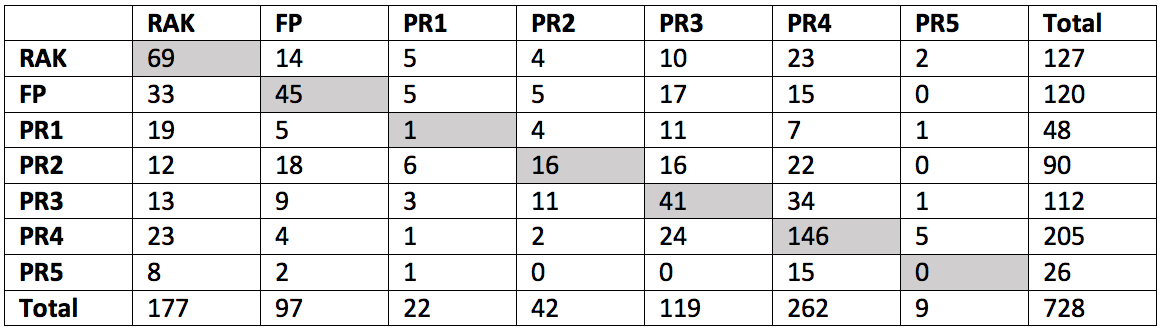
\includegraphics[width=.95\linewidth]{figures/thoeming_Table5}
	\centering
	\captionof{table}{Confusion Matrix Accuracy.}		
	\label{fig:Table5}
\end{figure}

%% this is FIGURE 9 Table 6
\begin{figure}[!htb]
	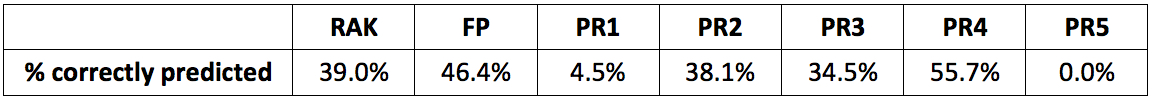
\includegraphics[width=.95\linewidth]{figures/thoeming_Table6}
	\centering
	\captionof{table}{Prediction Accuracy.}		
	\label{fig:Table6}
\end{figure}

\begin{figure}[!p] \label{fig:Fig4} 
	\begin{minipage}[b]{0.5\linewidth}
		\centering
		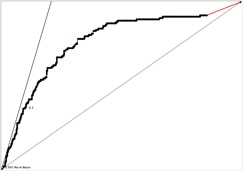
\includegraphics[width=.9\linewidth]{figures/thoeming_Fig4} 
		\caption{ROC (Receiver Operating Characteristic) Curve for RAK} 
	\end{minipage} 
	\begin{minipage}[b]{0.5\linewidth}
		\centering
		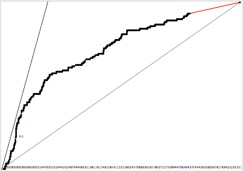
\includegraphics[width=.9\linewidth]{figures/thoeming_Fig5} 
		\caption{ROC (Receiver Operating Characteristic) Curve for FP} 
	\end{minipage} 
	\begin{minipage}[b]{0.5\linewidth}
		\centering
		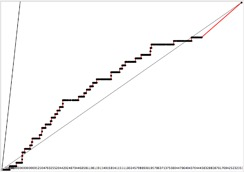
\includegraphics[width=.9\linewidth]{figures/thoeming_Fig6} 
		\caption{ROC (Receiver Operating Characteristic) Curve for PR1} 
	\end{minipage}
	\hfill
	\begin{minipage}[b]{0.5\linewidth}
		\centering
		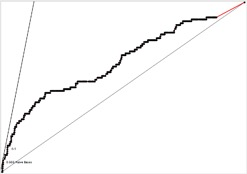
\includegraphics[width=.9\linewidth]{figures/thoeming_Fig7} 
		\caption{ROC (Receiver Operating Characteristic) Curve for PR2} 
	\end{minipage}
	\begin{minipage}[b]{0.5\linewidth}
		\centering
		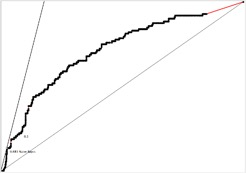
\includegraphics[width=.9\linewidth]{figures/thoeming_Fig8} 
		\caption{ROC (Receiver Operating Characteristic) Curve for PR3} 
	\end{minipage} 
	\begin{minipage}[b]{0.5\linewidth}
		\centering
		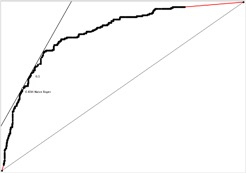
\includegraphics[width=.9\linewidth]{figures/thoeming_Fig9} 
		\caption{ROC (Receiver Operating Characteristic) Curve for PR4} 
	\end{minipage} 
	\centerline{\begin{minipage}[b]{0.5\linewidth}
		\centering
		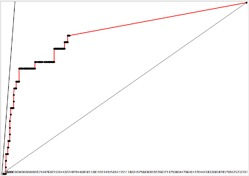
\includegraphics[width=.9\linewidth]{figures/thoeming_Fig10} 
		\caption{ROC (Receiver Operating Characteristic) Curve for PR5} 
	\end{minipage}}
\end{figure}
	
Two possibilities present themselves in these results. The first is that the data are not comprehensive enough for the identification of meaningful patterns, and the second is that there is no significant temporal variation in the crosses and inscriptions on the rune-stones. These results show the potential for the use of a Naïve Bayes Classifier in a way that may not be expected; it may just as easily be utilised to show a lack of classificatory potential.

%\section{Discussion and Conclusion}
Two\marginnote{{Discussion and Conclusion}} possibilities present themselves in these results. The first is that the data are not comprehensive enough for the identification of meaningful patterns, and the second is that there is no significant temporal variation in the crosses and inscriptions on the rune-stones. These results show the potential for the use of a Naïve Bayes Classifier in a way that may not be expected; it may just as easily be utilised to show a lack of classificatory potential.

The ease with which a Naïve Bayes Classifier can be put into use has been presented here, along with the methodology for doing so. Programs such as Orange, with their simple drag-and-drop GUI, require very little exposure to ‘actual math’. The outline for testing presented in this paper if used correctly will provide acceptable accuracy with which to make statistical conclusions about archaeological data. There are many situations for which a Classifier can be utilised, the most common of which have been presented above. Dating can be difficult for many reasons, i.e. a stylistic chronology cannot necessarily stretch to an entire artefact population, C14 dating can be prohibitively expensive for a large number of samples, etc. Other possibilities for Naïve Bayes Classification include classifying large numbers of samples into groups based on their combinations of attributes, or indeed, as identified above, doing the exact opposite of what the Classifier was designed for: identifying homogeneity. If nothing else, the ease with which the Classifier can be utilised and understood makes for an excellent avenue into the world of advanced statistical modelling for students of archaeology.
\myseparator
%\section{Acknowledgements}
For\marginnote{Acknowledgements} his assistance in the preparation of this manuscript, I would like to thank my supervisor Professor Roland Fletcher. His support in my endeavour to use this strange-sounding technique in my work is most appreciated, and without it, this would not have been attempted. The feedback I received at the National Archaeology Student Conference (NASC) in Adelaide 2014 also influenced the preparation of this manuscript, and was much appreciated. Finally, I must thank Jack Galilee, whose patience in explaining the basics of inferential and Bayesian statistics to a somewhat clueless archaeologist is much appreciated, convincing me that advanced statistics need to be a much more central part of an archaeological education. 


\begin{myabstract}
\foreignlanguage{swedish}{%
	Matematisk\marginnote{Abstract (Swedish)} analys blir allt mer användbart vid hantering av stora mängder arkeologisk data, tack vare de precisa och säkra resultat en sådan analys genererar. Den här artikeln diskuterar användningen av ett relativt nytt verktyg för att tolka och hantera arkeologisk data, Naiv Bayesiansk klassificering. Det ’Bayesianska’ angreppssättet presenterades först i början av 1990-talet av den arkeologiska statistikern Clive Orton  \parencites[139]{Orton_1992}[1]{Buck_1996}, trots att bristen på den tillgängliga beräkningsförmågan vid den tiden gjorde det påfallande svårt att använda denna typ av klassificering. Idag kan en Naiv Bayesiansk klassificering hanteras av alla som har tillgång till en dator, utan krav på några speciella datorkunskaper. Program så som Orange använder ett grafiskt gränssnitt som ett sätt att kringgå behovet av särskilda matematiska kunskaper om processen, användandet av detta program finns specificerat i artikeln. Naiv Bayesiansk klassificering är mest användbart vid försök att identifiera dolda mönster i stora mängder data, så som en databas med tusentals poster, och potentiella användningsområden kommer att illustreras här. 
	Den här artikeln presenterar en fallstudie där Naiv Bayesiansk klassificering används i ett försök att datera svenska vikingatida runstenar, vilka förblir odaterade med kontroversiella metoder. Två variabler identifierades genom att visa vissa spår av tidsmässig utveckling, de kristna korsen och runinskriptionerna på stenarna, och klassificeringsmetoden användes för att undersöka deras vidareanvändning.}

\keywords[Nyckelord]{Bayesiansk statistik, arkeologisk statistik, Naiv Bayesiansk klassificering, arkeologisk metodologi, kvantitativa metoder.}
\end{myabstract}
\printbibliography[heading=subbibnumbered] 
\label{thoeming:lastpage}
\closingarticle
